\documentclass[border=2pt]{standalone}
\usepackage[dvipsnames,svgnames,x11names]{xcolor}
\usepackage{tikz}
\usepackage{pgfplots}
\pgfplotsset{compat=1.18}
\usetikzlibrary{calc,arrows.meta,positioning,intersections,fit,shapes.geometric}
\usepgfplotslibrary{fillbetween}
\usepgfplotslibrary{groupplots}

\begin{document}
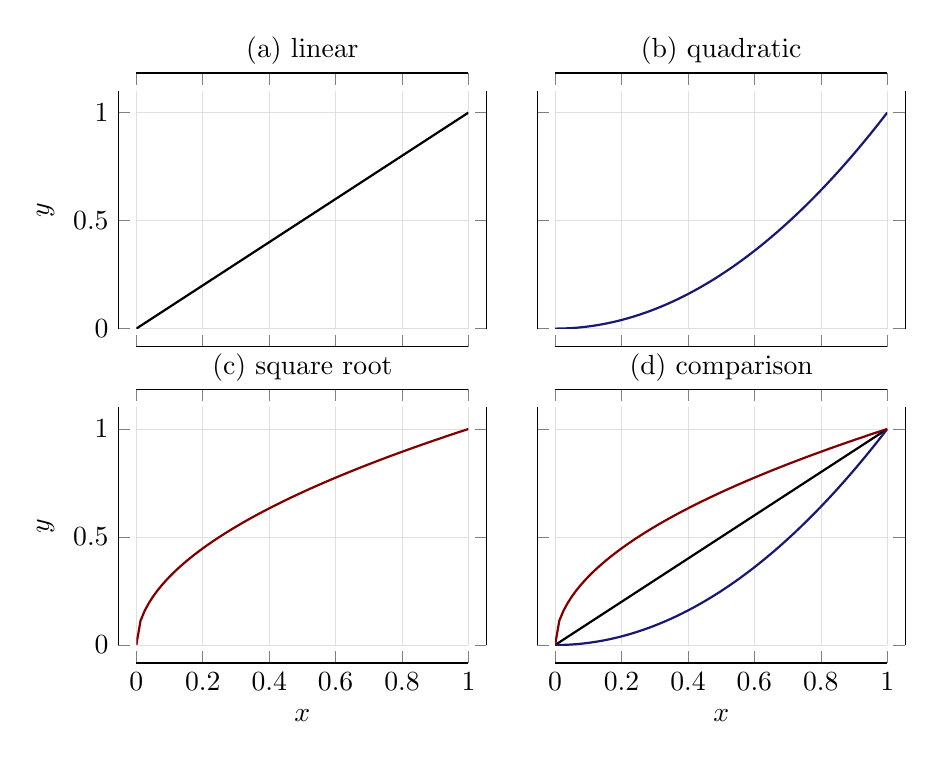
\begin{tikzpicture}
\begin{groupplot}[
  group style={group size=2 by 2,horizontal sep=1.1cm,vertical sep=1.0cm,xticklabels at={edge bottom},yticklabels at={edge left},xlabels at={edge bottom},ylabels at={edge left}},
  width=5.8cm,
  height=4.6cm,
  axis line shift=6.5pt,
  grid=major,
  grid style={gray!25,line width=0.2pt},
  xlabel={$x$},
  xmin=0,
  xmax=1,
  ylabel={$y$},
  ymin=0,
  ymax=1.1,
  legend style={draw=none,fill=none,cells={anchor=west}},
]
\nextgroupplot[title={(a) linear}]
\addplot+ [black,line width=0.8pt,mark=none,domain=0:1,samples=80] {x};
\nextgroupplot[title={(b) quadratic}]
\addplot+ [MidnightBlue,line width=0.8pt,mark=none,domain=0:1,samples=80] {x^2};
\nextgroupplot[title={(c) square root}]
\addplot+ [Maroon,line width=0.8pt,mark=none,domain=0:1,samples=80] {sqrt(x)};
\nextgroupplot[title={(d) comparison}]
\addplot+ [black,line width=0.8pt,mark=none,domain=0:1,samples=80] {x};
\addplot+ [MidnightBlue,line width=0.8pt,mark=none,domain=0:1,samples=80] {x^2};
\addplot+ [Maroon,line width=0.8pt,mark=none,domain=0:1,samples=80] {sqrt(x)};
\end{groupplot}
\end{tikzpicture}
\end{document}
